\subsubsection{Counterfactual policy reforms}
\label{sec:counterfactuals}

This paper delivers two kinds of counterfactual. The first kind is a change to
the \emph{location} of the single VAT registration threshold. I organise these
around two objects. The first is the \emph{anchor reform}: the actual increase of
the registration threshold from \pounds85{,}000 to \pounds90{,}000 that took
effect on 1~April 2024. This is a real, recent policy change, and I benchmark my
static costing of it directly against HM Revenue and Customs' own published
costing (Section~\ref{sec:results}). The second is a \emph{forward-looking sweep}
of alternative threshold locations spanning \pounds70{,}000 to \pounds120{,}000,
costed from the post-reform \pounds90{,}000 baseline. The anchor reform tells me
whether the model reproduces a costing I can check; the sweep then maps out the
fiscal menu of further location moves.

The second kind is a change to the \emph{shape} of the schedule:
Section~\ref{sec:cf_taper} delivers a \emph{graduated taper} that replaces the
\pounds85{,}000 notch with an effective rate that phases linearly from $0\%$ at
\pounds85{,}000 to the full $20\%$ at \pounds105{,}000. A schedule-shape change has
no single point of excess mass that a reduced-form bunching estimator can
forward-map; pricing it requires re-solving each firm's choice under a new,
continuous tax function, which the calibrated model lets me do.

Alongside these threshold-location reforms, the microsimulation assigns each firm a
cost parameter $\{A_i\}$ consistent with its observed turnover and inputs
(Section~\ref{sec:model}); I make no claim to identify it as a structural
primitive. Holding $\{A_i\}$ fixed, I replace the tax schedule $\tau(\cdot)$ with a
counterfactual policy, re-solve each firm's choice for a new optimal turnover
$y_i^{\text{new}}$, and re-aggregate the weighted choices into a counterfactual
turnover distribution.

\subsubsection{What the calibrated model adds}
\label{sec:cf_valueadded}

For the revenue cost of a pure threshold-\emph{location} change, a static
mechanical calculation already captures the first-order fiscal effect---the close
HMRC consistency check in Section~\ref{sec:results} comes from that
calculation---so I do not lean on the calibrated model there. Its distinctive
payoff is to price the reform a reduced-form estimator cannot: a change to the
\emph{shape} of the schedule, which has no single point of excess mass to
forward-map. I exploit this in Section~\ref{sec:cf_taper} to replace the notch
with a graduated taper. Along the way the model also simulates the full firm-size
\emph{distribution} under unobserved thresholds and separates optimisation from
frictions, neither of which the reduced form isolates. I exploit it again for a
second schedule-shape reform---a banded reduced rate for small firms
(Section~\ref{sec:results_rate}). A \emph{sector-specific} split rate for
labour-intensive services is feasible with the same machinery but is left to future
work (Section~\ref{sec:conclusion}).

\subsubsection{Frictions matter: a dynamic re-optimisation check}
\label{sec:cf_dynamic}

Before pricing the taper, I verify that the calibrated behavioural rule, not
frictionless optimisation, is the right tool---evidence that disciplines the
model. I re-solve the firm-size distribution under a threshold move
(\pounds85{,}000 to \pounds95{,}000) under two assumptions. In the
\emph{Pure-FOC} variant every firm re-optimises fully to its new FOC solution,
collapsing the old mass and re-forming it as a sharp double spike at the new
cutoff. The \emph{FOC+Uncertainty} variant adds a threshold-aware perturbation,
$y^{\text{unc}}_i = y^{\text{FOC}}_i\,(1+\varepsilon_i)$ with
$\varepsilon_i \sim \mathcal{N}(0, \sigma_\varepsilon^{2})$,
$\sigma_\varepsilon = 0.04$, capturing the frictions and imperfect foresight that
keep firms off the kink; this replaces the double spike with a rounded hump and
reproduces the observed pattern that only a minority reposition. The frictionless
variant materially overstates the response---the quantitative gap (mean turnover
\pounds1{,}488k versus actual \pounds1{,}130k) is stated in
Section~\ref{sec:results_structural}---so FOC+Uncertainty is the variant I carry
into the taper. Figure~\ref{fig:foc_dynamic} contrasts the two against the actual
distribution.

\begin{figure}[htbp]
\centering
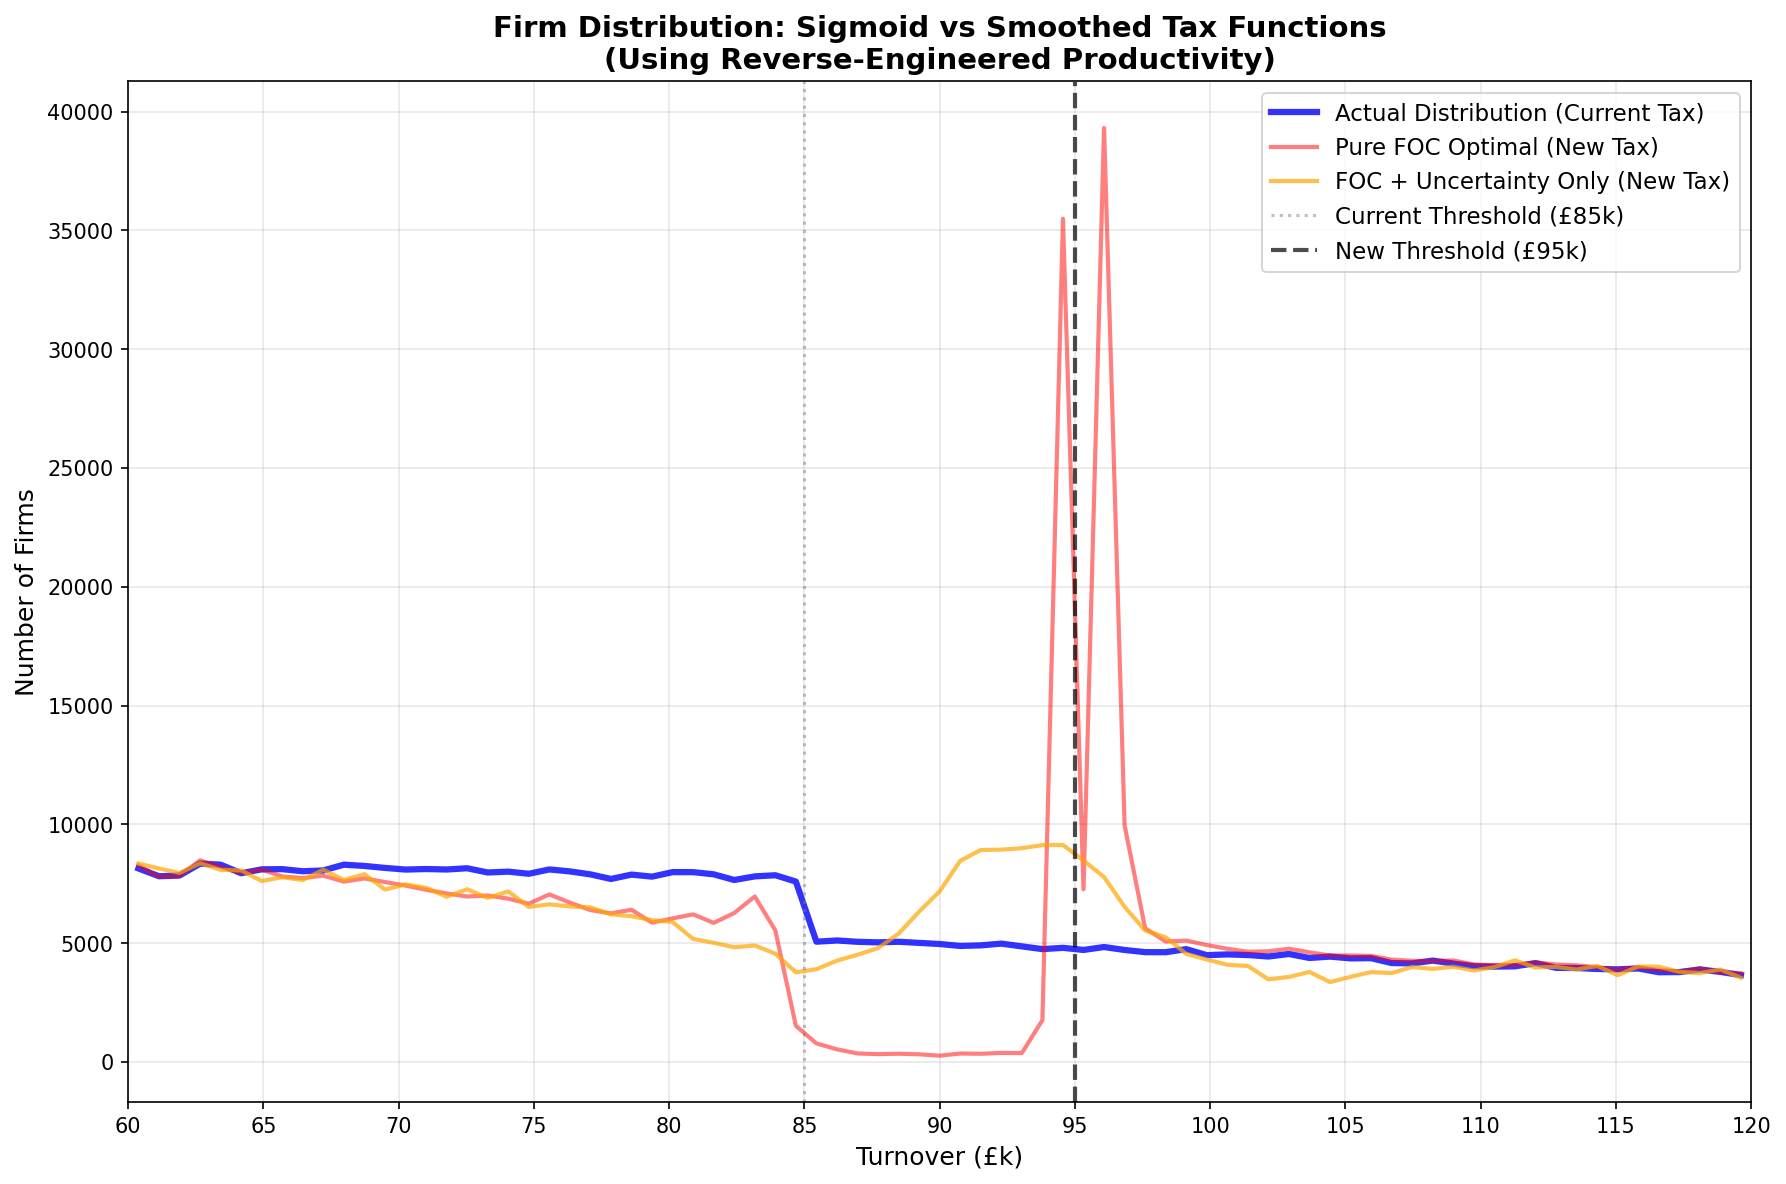
\includegraphics[width=0.9\textwidth]{figures/foc_dynamic_85kdata_full.png}
\caption{Dynamic re-optimisation under a new \pounds95{,}000 threshold, applied
to the \pounds85{,}000-era data. The \emph{Actual} distribution shows the
density step at the old \pounds85{,}000 threshold. The \emph{Pure-FOC} variant,
in which every firm re-optimises fully and frictionlessly, collapses the old mass
and re-forms it as a sharp double spike at the new \pounds95{,}000 threshold,
overstating the realised response. The \emph{FOC+Uncertainty} variant adds a
threshold-aware perturbation $\varepsilon \sim \mathcal{N}(0, 0.04^{2})$,
replacing the double spike with a smoothed hump around the new threshold that
matches the realised, partial nature of firm responses.}
\label{fig:foc_dynamic}
\end{figure}

\subsubsection{A graduated taper: the delivered schedule-shape reform}
\label{sec:cf_taper}

The dynamic experiment above still concerns a threshold-\emph{location} move,
for which the reduced form is a sufficient tool. I now use the calibrated model
for the task it alone can perform: pricing a change to the \emph{shape} of the
schedule. I replace the notch with a \emph{graduated taper}. Let $T_{0}$ denote the lower
edge of the taper band (the current registration threshold), $T_{1}$ its upper
edge, and $\tau_{\max}$ the standard VAT rate. Under the taper a firm with
turnover $y$ faces an effective rate
\begin{equation}
\tau_{\text{eff}}(y) =
\begin{cases}
0, & y < T_{0},\\[2pt]
\tau_{\max}\,\dfrac{y - T_{0}}{T_{1} - T_{0}}, & T_{0} \le y \le T_{1},\\[6pt]
\tau_{\max}, & y > T_{1},
\end{cases}
\label{eq:taper}
\end{equation}
so the effective liability phases linearly from $0$ at $T_{0}$ to the full rate
$\tau_{\max}$ at $T_{1}$. I implement the taper with $T_{0}=\pounds85{,}000$,
$T_{1}=\pounds105{,}000$ (a \pounds20{,}000 band) and $\tau_{\max}=0.20$. The taper eliminates the discrete jump in tax
liability that creates the notch: a firm that crosses \pounds85{,}000 no longer
faces VAT on its entire value added at once, only on the marginal slice implied by
its position in the band.

To price this reform I hold the calibrated firm cost parameters $\{A_i\}$ fixed
and re-optimise each firm's profit under the tapered $\tau(\cdot)$. Because
near-constant returns make the unconstrained optimum a knife edge, I re-optimise
over a bounded neighbourhood of each firm's observed turnover, consistent with the
partial, localised responses documented in Section~\ref{sec:results_structural}. The
crucial difference between the two schedules is the
\emph{local tax wedge} $y\,\tau'(y)$: under the notch this wedge is large and
concentrated at \pounds85{,}000 (it is what drives firms to bunch just below);
under the taper it is small and constant across the band, so the incentive to
suppress turnover largely disappears. The reduced-form bunching estimator cannot
evaluate this reform, because once the notch is replaced by a smooth schedule
there is no single point of excess mass to forward-map.

The quantitative results, distributional effect, and figure for the taper are
reported in Section~\ref{sec:results_taper}.

\subsubsection{Static versus behavioural evaluation}
\label{sec:cf_static_vs_behavioural}

I distinguish the dynamic, behavioural simulation above from a \emph{static}
counterpart. In the static approach, firm turnover is held fixed and the new
schedule applied mechanically, so revenue changes reflect only reclassification
across the threshold; this benchmark underlies both the anchor-reform check and
the threshold sweep. The behavioural FOC+Uncertainty simulation instead captures
the second-order offset from re-optimisation and is the relevant object for how a
reform reshapes the firm-size distribution. The revenue, firm-count, and
distributional results for the threshold-location reforms are reported in
Section~\ref{sec:results}.
